\documentclass{article}
\usepackage[pdftex]{graphicx}
\usepackage{amsmath}
\addtolength{\textwidth}{1in}
\addtolength{\oddsidemargin}{-.5in}
\setlength{\evensidemargin}{\oddsidemargin}


%\VignetteIndexEntry{Evidential Sample Size, Relative Risk, and Interval Interopaltion Using Likelihood Methods }

\title{Sample Size, Relative Risk, and Interval Interopaltion Using Evidence based Likelihood Methods}
\author{Sarah Fletcher\\ Vanderbilt University Biostatistics}

\usepackage{Sweave}
\begin{document}
\maketitle
\tableofcontents
\section{Introduction}

This package is based on the Likelihood framework and requires  a basic knowledge of the evidential paradigm.  For a breif introduction please refer to Royall [1] and  Blume [2].  The Likelihood framework focuses on itnerpreting data as statistical evidence, and uses likelihood ratios to measure the strength of statistical evidence of one hyposthesis over another.  

\section{Evidential Sample Size}

The likelihood paradigm defines evidence as strong, weak, and misleading, and these probabilities are the foundations of evidential sample size estimation.   Sample sizes are calculated such that the probability of strong evidence given N and k is less than the specified strong evidence bound. In other words $P(Strong Evidence | N, k) <0.80, 0.85, 0.90$.  These strong evidence bounds can be adjusted by the user but default to the above. 

 For the purpose of interpreting and communicating the strength of evidence, it is useful to divide the continuous scale of the likelihood ratio into descriptive categories, such as weak, moderate and strong evidence. 
Such a crude categorization allows a quick and easily understood characterization of the evidence for one hypothesis over another.
 Benchmark values of k = 8 and 32 have been suggested to distinguish between weak, moderate and strong evidence.  The function ss.mean() defaults to values of k=8 and 32, but can also be specified by the user.  The $P(Weak Evidence | N, k)$ can be interpreted as $1-P(Strong Evidence | N, k)$, since it is assumed that the $P(Misleading Evidence | N, k)$ is approximately 0.  These sample size calculations are modeled after methods presented by Strug [3].
 
The function ss.mean() will return a data frame containing all combination of values of k, S (Strong evidence), and delta (Effect size), and the resulting sample size to detect strong evidence in favor of one hypothesis over another.  

\subsection{Examples of ss.mean()}
\begin{Schunk}
\begin{Sinput}
> ss.mean(k=c(8,32),S=c(0.80,0.85), delta=c(.5,1.5))
\end{Sinput}
\begin{Soutput}
   k Strong.evidence Effect.size Sample.size
1  8            0.80         0.5   37.156254
2  8            0.85         0.5   44.196580
3  8            0.80         1.5    4.128473
4  8            0.85         1.5    4.910731
5 32            0.80         0.5   52.002551
6 32            0.85         0.5   59.779554
7 32            0.80         1.5    5.778061
8 32            0.85         1.5    6.642173
\end{Soutput}
\begin{Sinput}
> ss.mean(k=c(8,20,32),S=c(0.80,0.85,0.90), delta=c(.2,.5))
\end{Sinput}
\begin{Soutput}
    k Strong.evidence Effect.size Sample.size
1   8            0.80         0.2   232.22659
2   8            0.85         0.2   276.22862
3   8            0.90         0.2   340.42677
4   8            0.80         0.5    37.15625
5   8            0.85         0.5    44.19658
6   8            0.90         0.5    54.46828
7  20            0.80         0.2   294.12536
8  20            0.85         0.2   341.24509
9  20            0.90         0.2   408.94786
10 20            0.80         0.5    47.06006
11 20            0.85         0.5    54.59921
12 20            0.90         0.5    65.43166
13 32            0.80         0.2   325.01594
14 32            0.85         0.2   373.62222
15 32            0.90         0.2   443.03191
16 32            0.80         0.5    52.00255
17 32            0.85         0.5    59.77955
18 32            0.90         0.5    70.88511
\end{Soutput}
\begin{Sinput}
> 
\end{Sinput}
\end{Schunk}
\section{Evidential Relative Risk}
For a more thorough understanding of the conditional likelihood model for relative risk see Blume (reference [2], p. 2589) and for the full derivation see Royall (reference [1], p. 165).  In short, of interest is the $RR=(y1/n1)/(y2/n2)$, where n1 is the total number of i.i.d. $Bernoulli(\theta_1)$ observations required to obtain $n1-y1$ failures and $n2$ is the total number of i.i.d. $Bernoulli(\theta_2)$ observations required to obtain $n2-y2$ failures. Let $RR = \theta_1/\theta_2$ be the relative risk for a successful event in group 1 versus group 2. 

The function rr\_like() takes in values y1, n1, and y2, n2, and returns a likelihood object that can be plotted or used to find support intervals.  The variables lo and hi specifiy the plotting region, and default to 0 and 6 respectively. The variable points is the number of points in [0,1] to calculate likelihood (defaults to 1000), and the varaible scale, scales the maximum likelihood to 1 (defaults to TRUE).  If plot(rr\_like()) is called, a likelihood plot is returned with support intervals at k=8 and 32, but can be specified otherwise.  

\subsection{Examples of rr\_like()}

\begin{Schunk}
\begin{Sinput}
> rr <- rr_like(15, 45, 5, 29,hi=10)
> interval(rr, 8)
\end{Sinput}
\begin{Soutput}
$endpoints
[1] 0.8308308 5.7757758

$like
[1] 0.125
\end{Soutput}
\begin{Sinput}
> interval(rr, 32)
\end{Sinput}
\begin{Soutput}
$endpoints
[1] 0.6606607 8.5185185

$like
[1] 0.03125
\end{Soutput}
\begin{Sinput}
> plot(rr)
> 
\end{Sinput}
\end{Schunk}
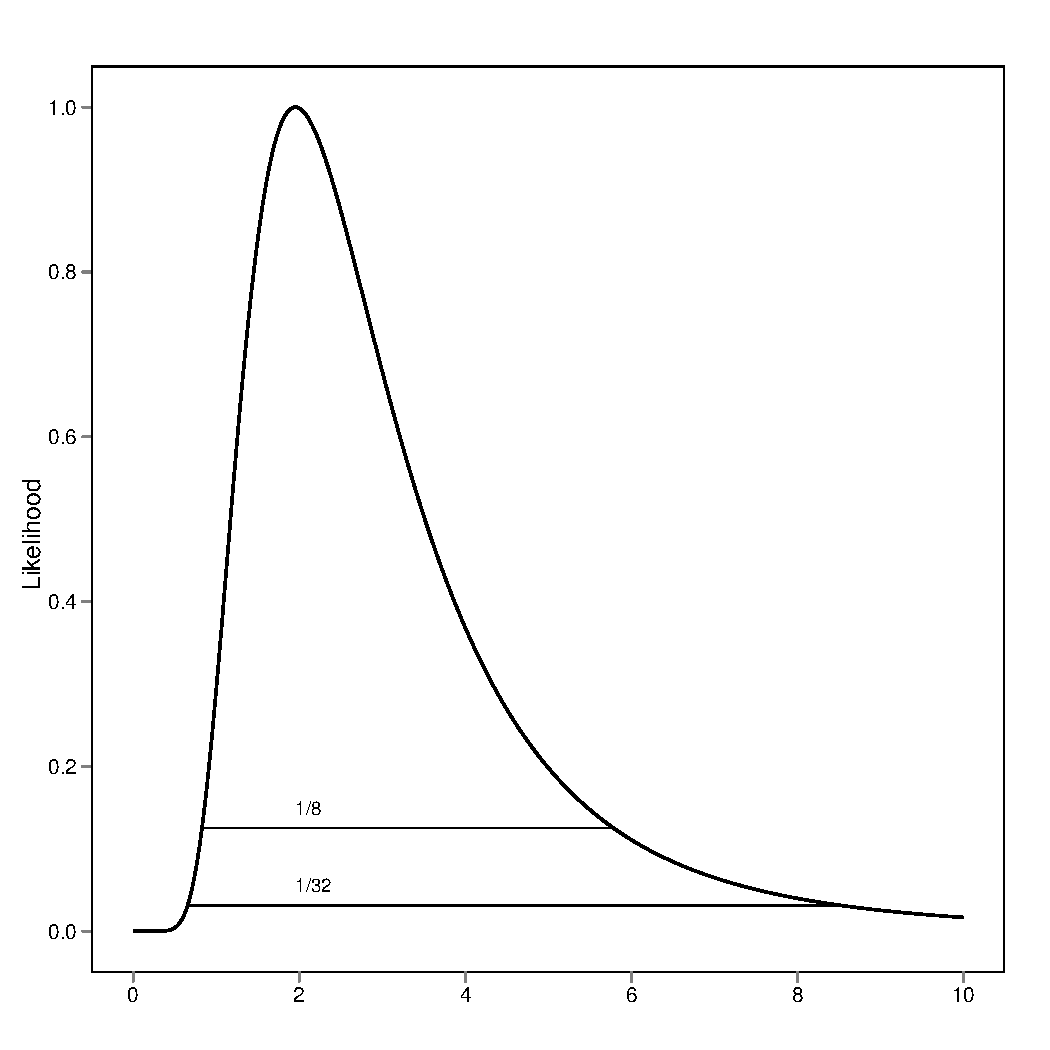
\includegraphics{rr.pdf}\section{Interval Interpolation}

If the user specifies less than 1000 points, the 1/8 and 1/32 plotting intervals (or other specified intervals) will
be interpolated from the likelihood object.  The function interpolate.likelihood() does not need to be specified and  the likelihood plotting function will call it if a user chooses to plot less than 1000 points.  The intervals will then be plotted in the usual way. 

\subsection{Examples of interpolated intervals}
\begin{Schunk}
\begin{Sinput}
> rr_10points<- rr_like(15, 45, 5, 29, hi=10, points=10)
> plot(rr_10points)
> 
\end{Sinput}
\end{Schunk}
\includegraphics{rr10points.pdf}\begin{Schunk}
\begin{Sinput}
> rr_20points<- rr_like(15, 45, 5, 29, hi=10, points=20)
> plot(rr_20points)
> 
\end{Sinput}
\end{Schunk}
\includegraphics{rr20points.pdf}
\begin{thebibliography}{9}
\bibitem{Royal97l} Royall RM. \emph{Statistical Evidence: A Likelihood Paradigm.}
   Chapman and Hall: London, 1997.
  \bibitem{Blume02} Blume JD, ``Tutorial in Biostatistics           %'
    Likelihood methods for meauring statistical evidence.", \emph{Statist. Med.} 21:2563--2599, 2002.
    \bibitem{Strug07} Strug LJ, Rohde C, Corey PN. ``An Introduction to Evidential Sample Size Calculations''
    \emph{The American Statistician} 61: 207--212, 2007.
\end{thebibliography}
\end{document}
